
\begin{figure}[h]
    \centering
    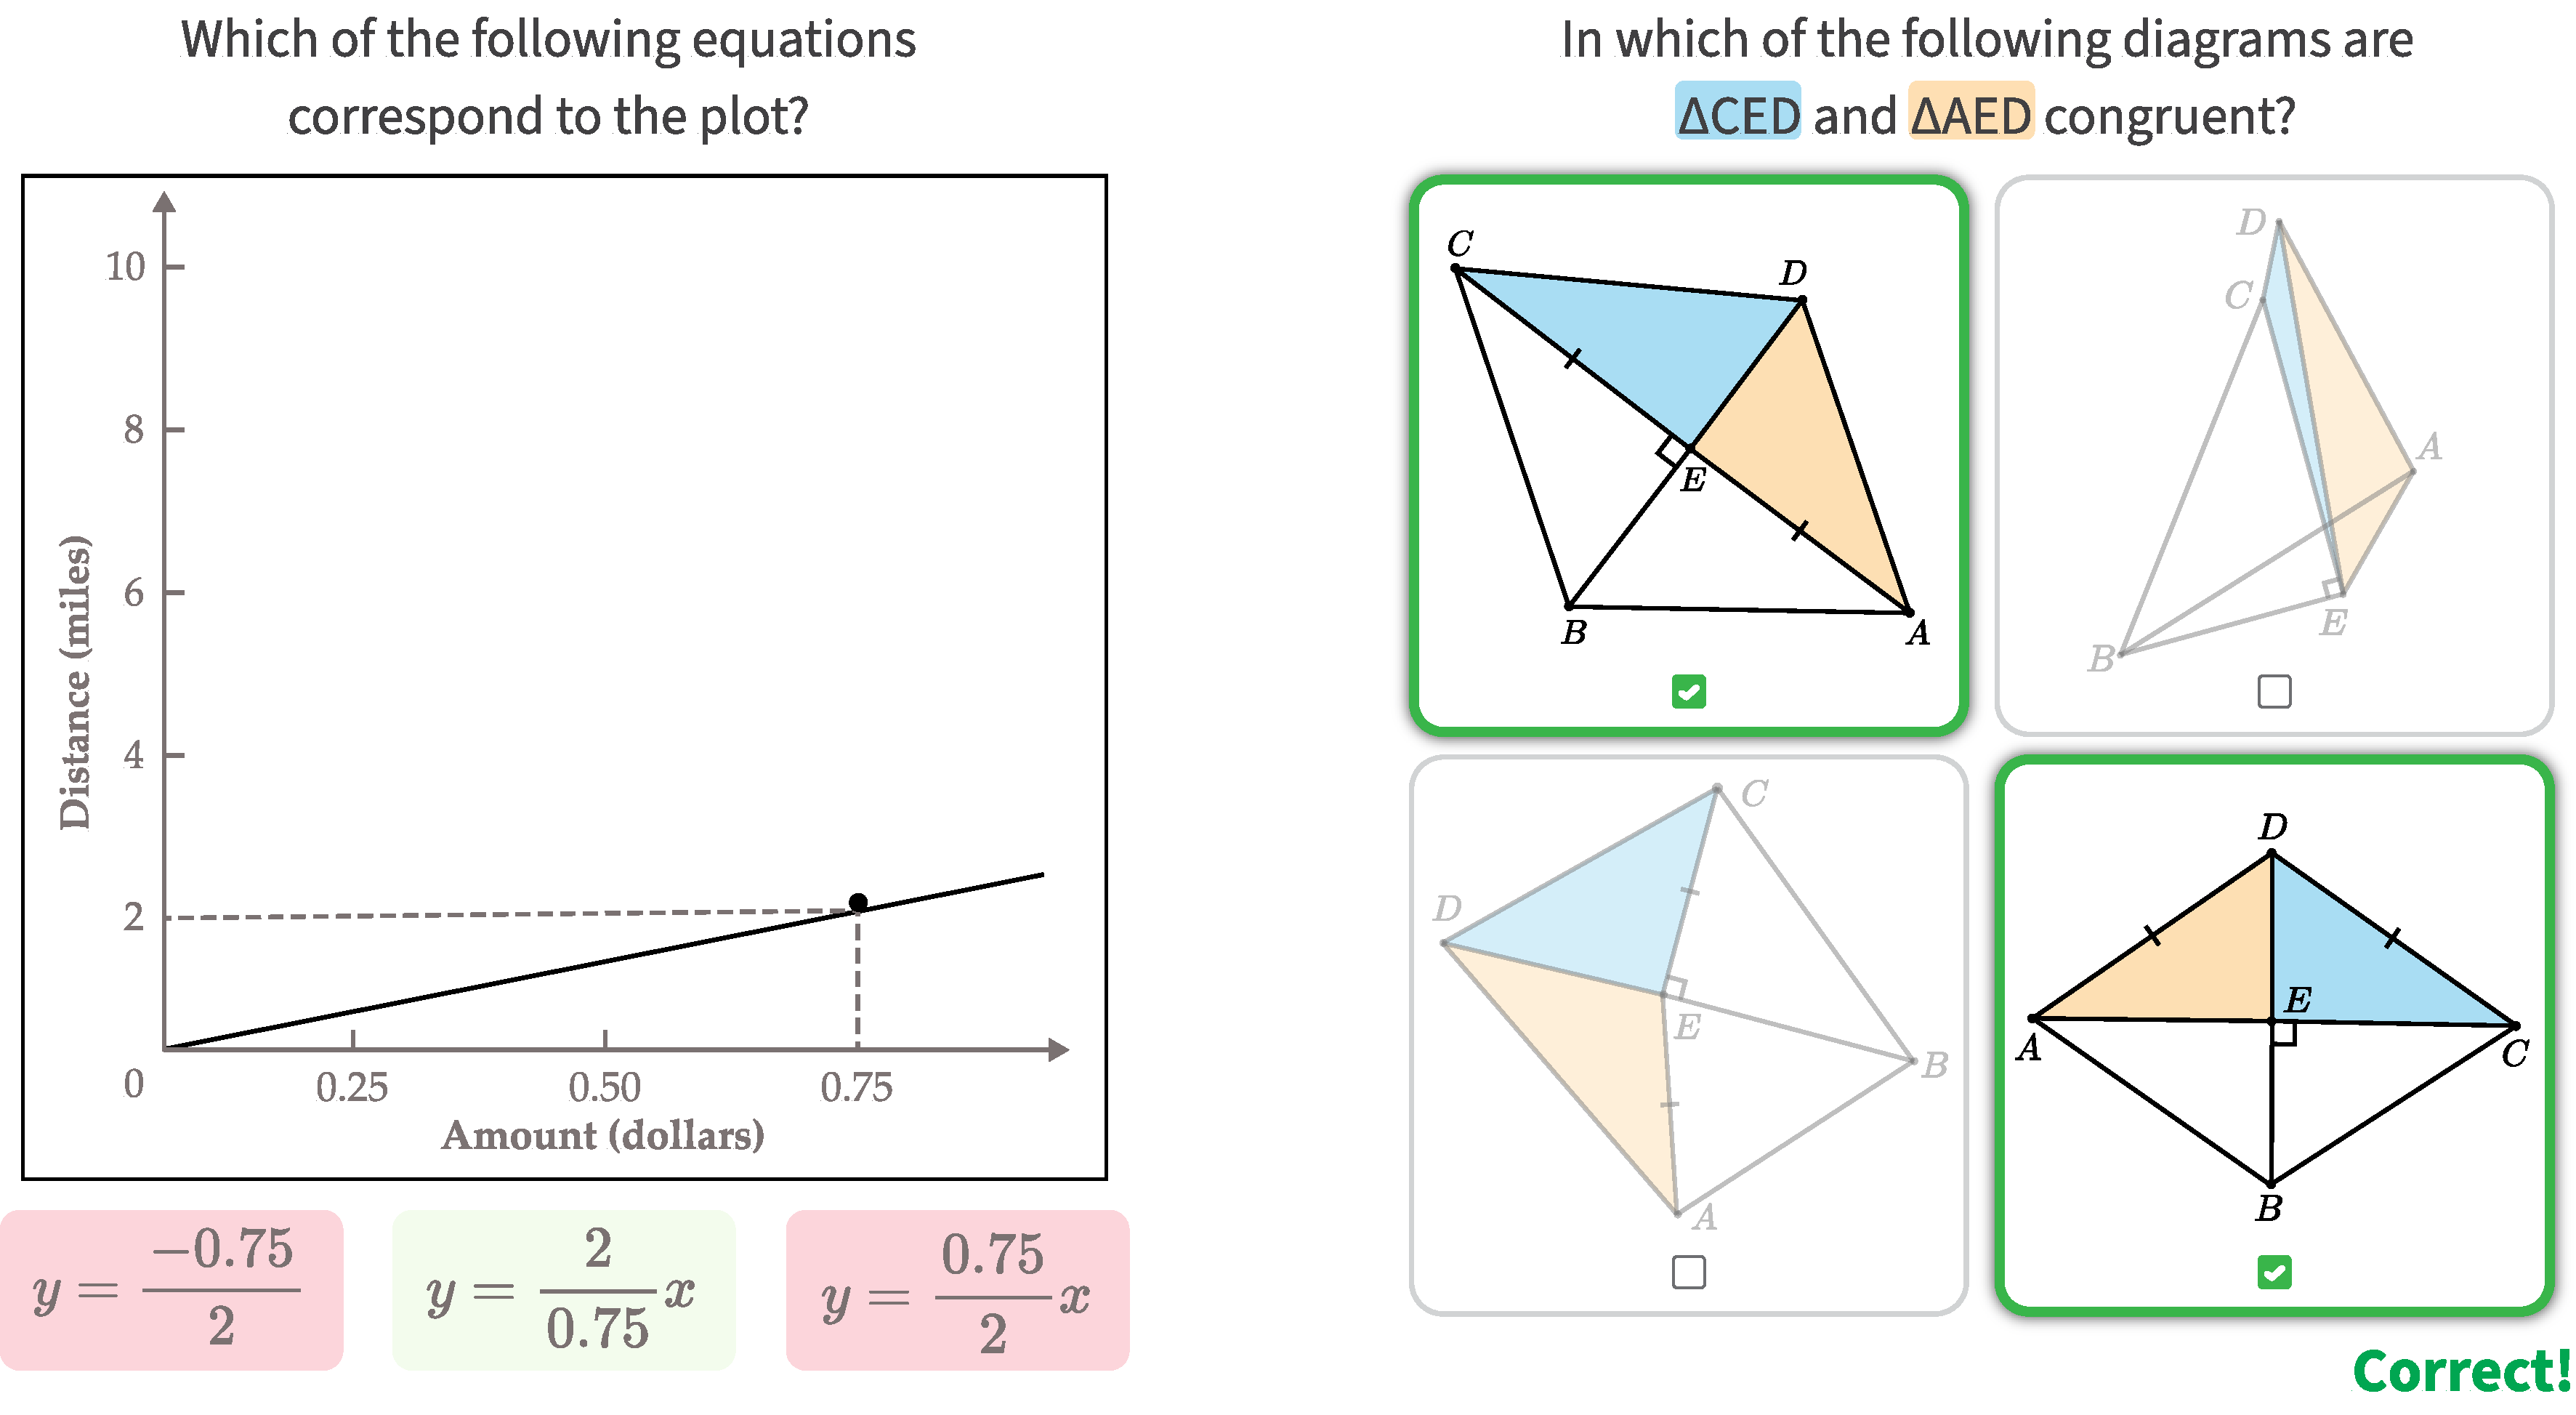
\includegraphics[width=0.88\linewidth]{assets/chapter-3/translation-problem.pdf}
    \caption{\textbf{left}: a translation problem that helps students discern the structure of linear equations (adapted from~\cite{perceptualLearning}). \textbf{right}: an \Edgeworth generated problem that trains student to recognize diagram configurations~\cite{Koedinger1990a} for triangle congruence.}
    \label{fig:translation-problem}
\end{figure}

\vspace{10pt}

\begin{figure}
    \centering
    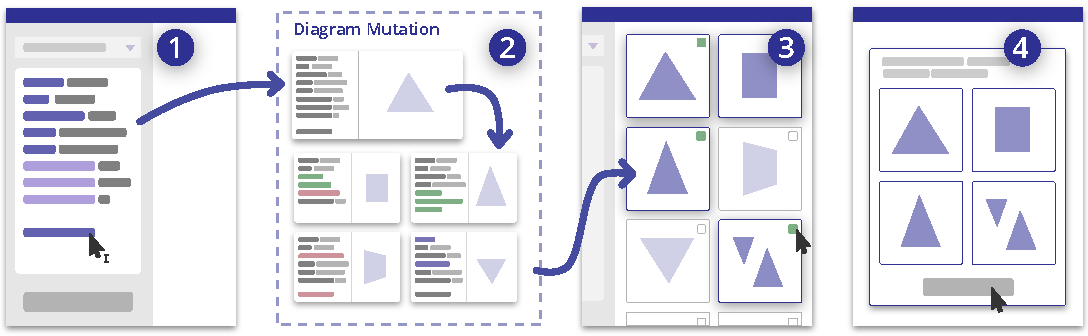
\includegraphics[width=\linewidth]{assets/chapter-3/edgeworth-teaser.pdf}
    \caption{\Edgeworth is a diagrammatic problem authoring tool that automatically generates diagram variations from a single diagram: \textmd{the author creates an example diagram~(\uilabel{1}), then \Edgeworth generates a myriad of diagram variations~(\uilabel{2}), from which the author selects diagrams~(\uilabel{3}) to form a diagrammatic multiple choice problem~(\uilabel{4}).}}
    \label{fig:teaser}
\end{figure}

\section{Introduction}

Effective use of visual representations requires a certain level of \emph{representational fluency} that's achievable through deliberate practice and repetition~\cite{metarepresentation, representationalFluency}. Recognizing how words, symbols, and diagrams relate to each other is an important first step of achieving fluency. Prior work has shown that these contrasting cases, \ie, discrimination and mapping, among representations significantly improve students' ability to translate among representations~\cite{perceptualLearning}.

To train students' representational fluency, educators often create problem sets that involve numerous contrasting cases of a particular visual representation. For instance, \cref{fig:translation-problem}~shows two examples of \emph{translation problems}, where the problem asks students to determine diagrammatic \emph{examples} and \emph{counterexamples} of a textual description and vice versa. Importantly, these examples and counterexamples have varying degrees of differences from the given diagram or text, and carefully picking examples on this spectrum has a big impact on learning~\cite{samenessAndDifference}.

Traditionally, educators author visual practice by drawing diagrams by hand. In formative interviews (\cref{sec:edgeworth-formative}), educators reported the vital role of visual practice in their instruction, but noted the tedium of authoring due to tool limitations, leading to fewer diagrams used than desired. Manual authoring can hardly keep up with the growth of STEM learners and demand for more visual practice.

As a first step towards scaling up visual practice authoring, we built \Edgeworth, a diagrammatic problem generator. \Edgeworth generates \emph{translation problems}, an effective type of visual practice~\cite{perceptualLearning} that ask students to determine diagrammatic \emph{examples} and \emph{counterexamples} of a textual/symbolic description (\cref{fig:translation-problem}). To help authors get the most out of one diagram, \Edgeworth contributes a ``build once, generate many'' authoring paradigm: Instead of manually editing diagrams to get variations, the author creates a single diagram and \Edgeworth automatically generates diagram variations (\cref{fig:teaser}\uilabel{1}\uilabel{2}). The interaction design of \Edgeworth allows the author to visually select diagram variations to rapidly form translation problems (\cref{fig:teaser}\uilabel{3}\uilabel{4}). Given the diversity of instructional contexts in STEM, we designed \Edgeworth to be domain-agnostic: it uses a generic program mutation technique~(\cref{sec:edgeworth-mutation}) to change the author-provided diagram to produce variations. 

In this chapter, we discuss formative interviews that drove the design of \Edgeworth{} and then walk through the technical implementation of \Edgeworth.

\section{Formative interview}

\label{sec:edgeworth-formative}

We conducted semi-structured interviews with 6 educators to understand how they author, use, and maintain diagrammatic problems. We recruited participants based on their background in education and usage of diagrams in their work. Selected participants work as secondary school teachers, university professors, teaching assistants, and competitive math coaches. All participants (P1--6) indicated that they have experience creating instructional material, authoring problems, and/or developing online courses that include visual content. Example interview questions include what roles diagrams play in the participant's educational materials, how students interact with diagrams, and how diagrams are authored and maintained. The full interview protocol is included in supporting files.

Participants reported the usage of diagrams to build conceptual understanding and emphasized the need for deliberate practice to acquire representational fluency. Traditional educational materials, especially in higher education, tend to emphasize \quotei{procedures, memorization, and symbolic manipulation} (P6).  Similarly, teachers such as P1 suffer from \quotei{the curse of knowledge} of teaching visual fluency: teachers tend to \quotei{under-train} students and they struggle to use visuals for problem-solving.  As a result, students often become \quotei{symbolically good} and do not develop \quotei{good conceptual understanding} (P3). Visuals like diagrams and graphs provide alternative representations that help students \quotei{develop intuition} (P3) and \quotei{become better problem-solvers} (P4). To improve their instruction, all of our participants (P1--6) attempt to incorporate more diagrams in their instructional materials. Some also ask students to draw, annotate, and explain diagrams (P1, P2, P6). P2 encourages students to learn \quotei{multiple representations} and makes diagrams central to their math and programming curricula. When students practice with diagrams, teachers also gain richer feedback on students' level of understanding, and \quotei{learned more from this [student-drawn diagram] than 10 similar problems without the pictures} (P6).

While the benefits of and need for diagrammatic practice are clear, participants reported that tool limitations led to manual and repetitive authoring experience. Because participants typically create many problems and iterate on their content often, they face a trade-off when authoring visual content: more visuals are beneficial for learning but are time-consuming to create and modify. When authoring practice problems, P1 struggled to \quotei{create simple shapes by myself} and always ended up \quotei{copy-pasting and searching online} repeatedly. Similarly, P6 reported that they \quotei{get online images for pre-made resources, but whenever I want something a little custom, it’ll take a lot of time.} To streamline the visual authoring process, P2 and P5 developed custom pipelines for authoring problem sets and quizzes using existing programming tools. Like the problems described by prior research on diagramming tool usability~\cite{naturalDiagramming}, these tools often lack support for \quotei{high-level tweaking of my diagrams} (P2) and \quotei{are a pain to use because the language is not semantic and hard to use for non-programmers} (P5). Participants showed us many examples of tedious changes necessary to create diagram variations.

From the results, we derived the following design requirements for tool design to address participants' needs:

\begin{enumerate}[label=\textbf{D\arabic*}]
    \item\label{req:fluency} Address the need for practicing representational fluency
    \item\label{req:variation} Simplify the workflow for generating diagram variations
    \item\label{req:layout} Obviate the need to attend to low-level diagramming details
\end{enumerate}



\section{System Design of \Edgeworth}
\label{sec:edgeworth-system-design}


\Edgeworth realizes the design goals from \cref{sec:edgeworth-formative} by: 1) providing a domain-agnostic workflow for rapidly authoring diagrammatic practice problems (\ref{req:fluency}), 2) automatically suggesting numerous diagram variations of a single example diagram and allowing the author to visually select from the variations (\ref{req:variation}), and 3) fully automating the layout for all diagram variations (\ref{req:layout}). \cref{fig:edgeworth-interface} walks through the user interface of \Edgeworth, a simple and clean design that encapsulates the ideas above.

In \cref{sec:edgeworth-workflow}, we demonstrate the workflow of \Edgeworth by showing how to author an example diagrammatic problem in Euclidean geometry. We then describe \Edgeworth's approach to diagram layout in \cref{sec:edgeworth-layout} and how it generates diagram variation in \cref{sec:edgeworth-mutation}. 

% Finally, we discuss the limitations of the current implementation in \cref{sec:limitations}.

\begin{figure}
    \centering
    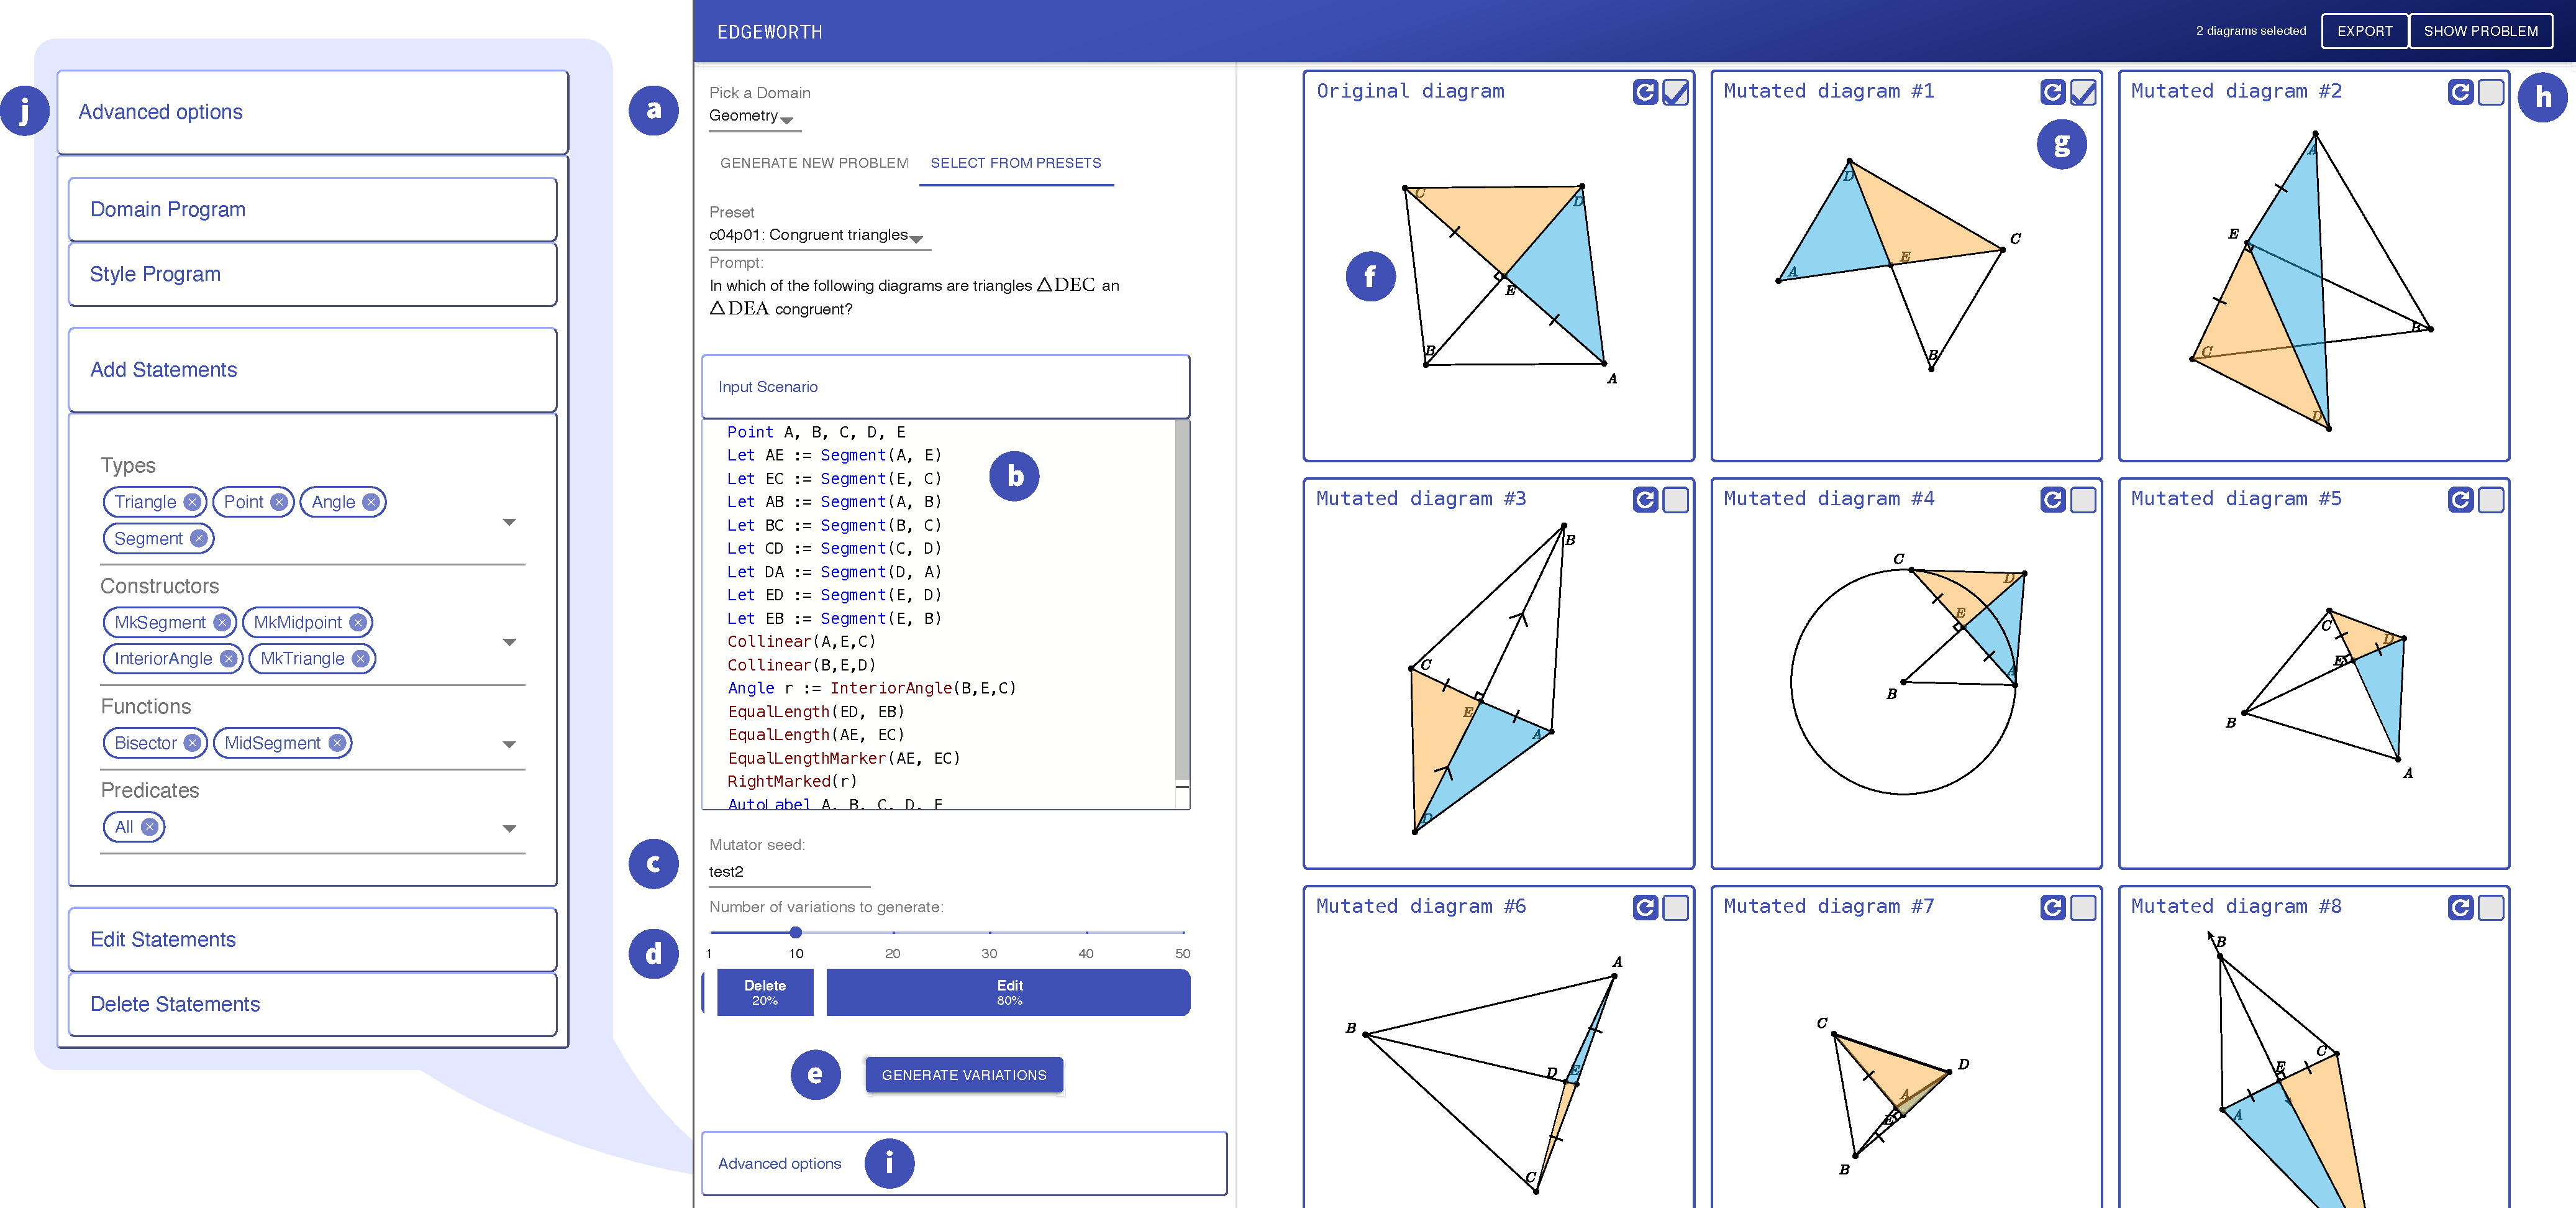
\includegraphics[width=\linewidth]{assets/chapter-3/edgeworth-ui-new.pdf}
    \caption{\textbf{The user interface of \Edgeworth.} \textmd{The author first provides a textual prompt~(\uilabel{a}) as an input scenario in \Substance notation~(\uilabel{b}). Then, clicking ``Generate Variations''~(\uilabel{e}) generates the specified number of diagram variations~(\uilabel{d}) at random based on a string seed and weights on Add, Delete or Edit mutations~(\uilabel{c}). In the diagram panel, the top-left diagram~(\uilabel{f}) corresponds to the input scenario and the rest are diagram variations generated by \Edgeworth. The author can visually select diagrams~(\uilabel{g}) to assemble a diagrammatic multiple-choice problem~(\uilabel{h}). If needed, the author can fine-tune the mutator using ``Advanced options'' (\uilabel{i}\uilabel{j}}). }
    \label{fig:edgeworth-interface}
\end{figure}

\subsection{Author Workflow}
\label{sec:edgeworth-workflow}

In this section, we use an example from high school geometry to demonstrate the process of creating a problem in \Edgeworth. 

\subsubsection{Create an example diagram} 
\label{sec:create-scenario}

The author wants to write a problem about triangle congruence to assess students' understanding of the \textit{Side-Angle-Side} (SAS) rule. They want to create a translation problem including one diagram where the SAS rule is satisfied and three others where it is not. The author first describes an example diagram (\cref{fig:edgeworth-interface}\uilabel{b}) where this rule is satisfied. They construct a scenario involving two triangles: $\triangle DEC$ and $\triangle DEA$ share one side $DE$ and have two equal sides $EC$ and $EA$. $\angle CEB$ indicates that $AC$ and $BD$ are perpendicular and therefore $\angle DEC = \angle DEA$. Therefore, $\triangle DEC$ and $\triangle DEA$ are congruent by the SAS rule. Given this description, \Edgeworth lays out the diagram automatically (\cref{fig:edgeworth-interface}\uilabel{f}). 

% \Edgeworth mutates this scenario to create variations that may or may not satisfy the SAS rule, and the author can select from these variations to create their translation problem. While \Edgeworth requires an example scenario, it does not require it to be correct or incorrect. The choice of this scenario is specific to the format of translation problems in this problem set. Constructing the example first guarantees that there will be at least one correct choice in the problem. If the author starts with an incorrect scenario, \Edgeworth may still mutate it to create a correct choice, but it is not guaranteed.

\subsubsection{Select from \Edgeworth-generated diagrams}
\label{sec:select-diagrams}

Now the author can use \Edgeworth to mutate the example diagram by clicking ``Generate Variations'' (\cref{fig:edgeworth-interface}\uilabel{e}). \Edgeworth performs mutations on the example scenario and generates a grid of diagram variations. The grid is designed to give the author an overview of the mutation results, and diagrams are prominent in each cell to facilitate faster visual selection. The top-left cell in the grid will always display the original example diagram (\cref{fig:edgeworth-interface}\uilabel{b}\uilabel{f}), and the rest correspond to mutation results.

By inspecting each diagram in the grid, the author can determine if it is a good fit for their translation problem. If so, they click the top-right checkbox (\cref{fig:edgeworth-interface}\uilabel{g}) to include the diagram in the problem.

\subsubsection{Preview and export the problem}
After the author picks a sufficient number of diagrams (4 in this case), they can preview the translation problem by clicking ``Show Problem'' (\cref{fig:edgeworth-interface}\uilabel{h}), which displays an interactive multiple-choice widget. If the author is satisfied, they can click ``Export'' to download the diagrams and metadata to use the problem in their context. \Edgeworth exports to Scalable Vector Graphics (SVG) images for static media, source programs for interactive use, and detailed mutation trace metadata for comprehensive analysis and reference purposes.

\subsection{Diagram Notation and Layout}
\label{sec:edgeworth-layout}

\Edgeworth is built on \Penrose~(\cref{chp:penrose}). Compared with alternatives, \Penrose offers two distinct advantages: (1) a high-level diagram notation that's easy for authoring and (2) an automatic layout engine. As discussed in \cref{chp:penrose}, a diagram in \Penrose consists of a textual description of the diagram content (\Substance) and a reusable layout stylesheet (\Style). As a reminder, \cref{fig:cocl2-example} shows the three kinds of \Substance statements: type statements (\eg \sub{Carbon c}) declare new objects; constructors (\sub{Bond b1 := SingleBond(c, cl1)}) create new objects from existing objects; and predicates (\sub{ZeroDots(c)}) indicate relations among objects. 

% \begin{wrapfigure}{r}{0.5\textwidth}
\begin{figure}[H]
    % \begin{center}
    \centering
    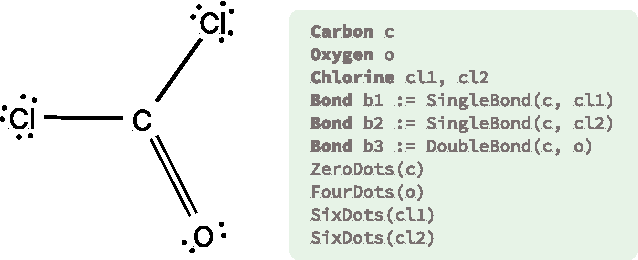
\includegraphics[width=.6\linewidth]{assets/chapter-3/cocl2-example.pdf}
    % \end{center}
    \caption{\textmd{Diagram and \Substance notation for the Lewis structure of phosgene (\ensuremath{\mathrm{COCl_2}}).}}
    \label{fig:cocl2-example}
\end{figure}

The current \Edgeworth implementation builds on \Penrose's geometry, chemistry, and graph \Style for diagram layout. Since the existing \Style stylesheets are primarily used to generate a few human-written examples, they lack coverage for variations of \Substance descriptions required by \Edgeworth. To this end, we improved \Style, diagram examples, and new standard library functions to \Penrose to accommodate \Edgeworth.

\Edgeworth is the first application of \Penrose that concurrently optimizes and renders a grid of multiple diagrams. Therefore, we have made significant updates to \Penrose to support \Edgeworth's use case. To make \Edgeworth a performant client-side web application for interactive use, we have migrated from Haskell to TypeScript and made various performance improvements to efficiently run tens of layout optimization jobs in a single session. Compared to the state of \Penrose at the publication of \citet{penrose}, the development of \Edgeworth has helped improve the performance of the system by 100$\times$.


\subsection{Program Mutation}
\label{sec:edgeworth-mutation}

% what is program mutation and why it's a good fit
\Edgeworth generates diagram variations by mutating the example diagram written in \Substance. 
% what the operators are
We purposely designed the system to include a small set of simple and type-safe mutation operations. Similar to generic tree-editing algorithms~\cite{gumtree}, \Edgeworth supports 3 kinds of mutation operators: \textbf{Add}, \textbf{Delete}, and \textbf{Edit}. \textbf{Add} appends a statement. \textbf{Delete} removes a statement and all other references to that statement. 

Since compilation errors in \Substance will not produce diagrams, \textbf{Edit} involves one of the type-safe patterns listed below. Each \textbf{Edit} pattern contains a \emph{guard} and an \emph{action}. The guard checks if the operator is applicable to the given \Substance statement, and the action performs the mutation. For instance, \textbf{Replace Arguments} is only applicable when the current context has existing variables of the desired type. 
\begin{itemize}[leftmargin=*]
    \item \textbf{Swap Arguments} reorders the arguments passed into a statement; \eg if \sub{A} and \sub{B} are \sub{Triangle}s:\\
            \sub{Similar(A, B)} $\rightarrow$ \sub{Similar(B, A)}
    \item \textbf{Replace Arguments} replaces the arguments passed into a statement with other arguments defined in scope; \eg if \sub{A, B, C, D} are \sub{Point}s:\\
            \sub{s := MkSegment(A, B)} 	$\rightarrow$ \sub{s := MkSegment(C, D)}
    \item \textbf{Replace Function} replaces a statement with a different statement that takes the same arguments; \eg if \sub{T} is a \sub{Triangle} and \sub{E} is an \sub{Angle}:\\
            \sub{Equilateral(T)} $\rightarrow$ \sub{Scalene(T)} \\
            \sub{Segment s := Bisector(E)} $\rightarrow$ \sub{RightAngleMarked(E)}
\end{itemize}

% one-col
\begin{algorithm}
\caption{The \Edgeworth mutation algorithm. }\label{alg:mutation}
\begin{algorithmic}[1]
\Function{Generate}{$p, \ell, h, a, d, e, A, D, E$}
\State $p' \gets p$
\State $n \gets \text{uniform random integer between $\ell$ and $h$}$\label{line:mutations}
\For{$i$ \textbf{from} $1$ \textbf{to} $n$}
    \State $x \gets \text{uniform random real between $0$ and $a + d + e$}$\label{line:kind}
    \If{$x < a$}
        \State $m \gets \textsc{RandomAdd}(A, p')$\label{line:add}
    \ElsIf{$x < a + d$}
        \State $m \gets \textsc{RandomDelete}(D, p')$\label{line:delete}
    \Else
        \State{$s \gets \text{uniform random element of $\textsc{Statements}(p')$}$}\label{line:statements}
        \State{$m \gets \textsc{RandomEdit}(E, s)$}\label{line:edit}
    \EndIf
    \State $p' \gets \textsc{Mutate}(p', m)$
\EndFor
\State \textbf{return} $p'$
\EndFunction
\end{algorithmic}
\end{algorithm}
% one-col

Algorithm~\ref{alg:mutation} shows how the \Edgeworth mutator works, at a high level. In addition to the input \Substance description $p$, \Edgeworth also takes a number of user-defined configuration parameters: (1) a number of variations to generate (the number of times \textsc{Generate} is called); (2) a range of mutation counts per variation (the input variables $\ell$ and $h$); (3) weights for \textbf{Add}, \textbf{Delete}, and \textbf{Edit} operations (the input variables $a$, $d$, and $e$ respectively); and (4) filter sets $A$, $D$, and $E$ which limit the set of mutations that the \textbf{Add}, \textbf{Delete}, and \textbf{Edit} operations can produce.

% how the mutator produces mutants
Given an example diagram, \Edgeworth performs several rounds of mutation generation. Each round results in a series of mutations that alter the input to produce a variation. The number of mutations (line~\ref{line:mutations}) is bounded by the configuration parameters.

To generate a single mutation, \Edgeworth makes a weighted choice (line~\ref{line:kind}) of the mutation kinds and enumerates all possible mutations for the chosen kind: \textbf{Add} enumerates all possible statements to add (line~\ref{line:add}); \textbf{Delete} randomly deletes an existing statement (line~\ref{line:delete}); \textbf{Edit} enumerates all possible edits for all statements (line~\ref{line:statements}) and picks one of them randomly (line~\ref{line:edit}). The randomness of \Edgeworth is controlled by a single random generator seed.

Users can specify filter sets under the ``Advanced options'' section of the UI, shown in \cref{fig:edgeworth-interface}\uilabel{i}\uilabel{j}. The filters default to ``All,'' which indicates that the mutator may change any statement in the example diagram. While this precise configuration may be useful, we ended up not using them in our evaluation (\cref{chp:edgeworth-eval}) and instead achieving our results using only \Edgeworth's simpler core set of configuration options, i.e., weights on mutation operators.

\section{Limitations}
\label{sec:limitations}

\subsection{Domains of instruction}
\label{sec:extension}

As shown in \cref{sec:edgeworth-mutation}, the design of the \Edgeworth mutator is domain-agnostic, as the mutation operators do not require any domain-specific knowledge to produce mutants. However, improving the layout stylesheet requires domain expertise. Therefore, future \Edgeworth authors may not have the technical background or the time to invest in a new \Penrose stylesheet, which might prohibit them from using \Edgeworth if the domain is not well supported by the \Penrose ecosystem. In practice, as noted by \citet[Section~5]{penrose}, the effort to build \Penrose stylesheets for new domains is only necessary once per domain and not once per diagram or problem.

\subsection{Numerical and textual variations}

\Edgeworth cannot produce numerical and textual variations like traditional problem generators~\cite{CTAT, ASSISTment} do. It is, however, possible to build this functionality on top of \Edgeworth to produce further problem variations. \cref{sec:problem-generation} further discusses this possibility in the context of existing template-based problem generation tools.

\subsection{Usability of UI components}

The design presented in \cref{sec:edgeworth-system-design} focuses on generating diagram variations and selecting diagram mutants to create problems. Here are some elements of the \Edgeworth tool that are not contributions of this paper, but may limit \Edgeworth's usability in practice: We use the \Substance language and \Penrose's textual interface without modification. Any limitations of \Substance and its UI are inherited by \Edgeworth. We use standard Material UI elements\footnote{\url{https://mui.com/}} to allow users to configure \Edgeworth (\eg a standard text box for changing diagram variations in \cref{fig:edgeworth-interface}\uilabel{c}). While these components might be usable as-is, they are not designed explicitly for the problem authoring workflow. 


\section{Translation Problem Dataset}
\label{sec:edgeworth-case-studies}

\begin{figure}[h]
    \centering
    % \includegraphics[width=\linewidth]{assets/problem-samples.pdf}
    \includegraphics[width=\linewidth]{assets/chapter-3/problem-samples.pdf}
    \caption{We used \Edgeworth to recast real-world problems as diagrammatic translation problems. Left: \textmd{Determine if triangles are congruent.}  Middle: \textmd{Identify the correct Lewis structure for hydrogen cyanide.} Right: \textmd{Identify graphs with Euler circuits.}}
    \label{fig:edgeworth-problems}
\end{figure}


% motivation
\Edgeworth's mutation-based approach is domain-agnostic: it simply applies generic program mutations on any \Substance program. Through collecting a dataset of translation problems in Euclidean geometry, general chemistry, and discrete mathematics, we evaluate if this approach is expressive enough for different instructional contexts in STEM. The 3 domains are selected based on their ubiquity in STEM education and visual representations. All three domains have a wide audience in K-12 and higher education, making them rich sources for existing instructional materials. Each domain has canonical visual representations that are explicitly taught to students. Therefore, students can benefit from visual practice in these domains.

% procedure
We choose problems from existing textbooks or online courses and follow the procedure outlined in \cref{sec:edgeworth-workflow} to recast each problem. 

% All problems are included in supporting files. 

\subsection{Summary Statistics}
\label{sec:edgeworth-case-studies-summary}

In the case studies, we reproduced 31 problems in total. Since creating the example diagram (\cref{sec:create-scenario}) took the most time in this process, we report statistics on the example diagrams here. 

On average, \Edgeworth's diagram notation is compact and simple. The description for example diagrams are 14.7 lines of code ($\sigma = 4.57$) and 109.9 tokens ($\sigma = 48.6$). In contrast, the average SVG source of these same diagrams have 454.7 lines of code ($\sigma = 184.3$) and 1290.4 tokens ($\sigma = 650.4$). This indicates that \Edgeworth provides a concise and compact textual representation of diagrams across all three domains.

\subsection{Euclidean Geometry}
\label{sec:edgeworth-geometry}

% one-col 
\begin{figure}[h]
    \centering
    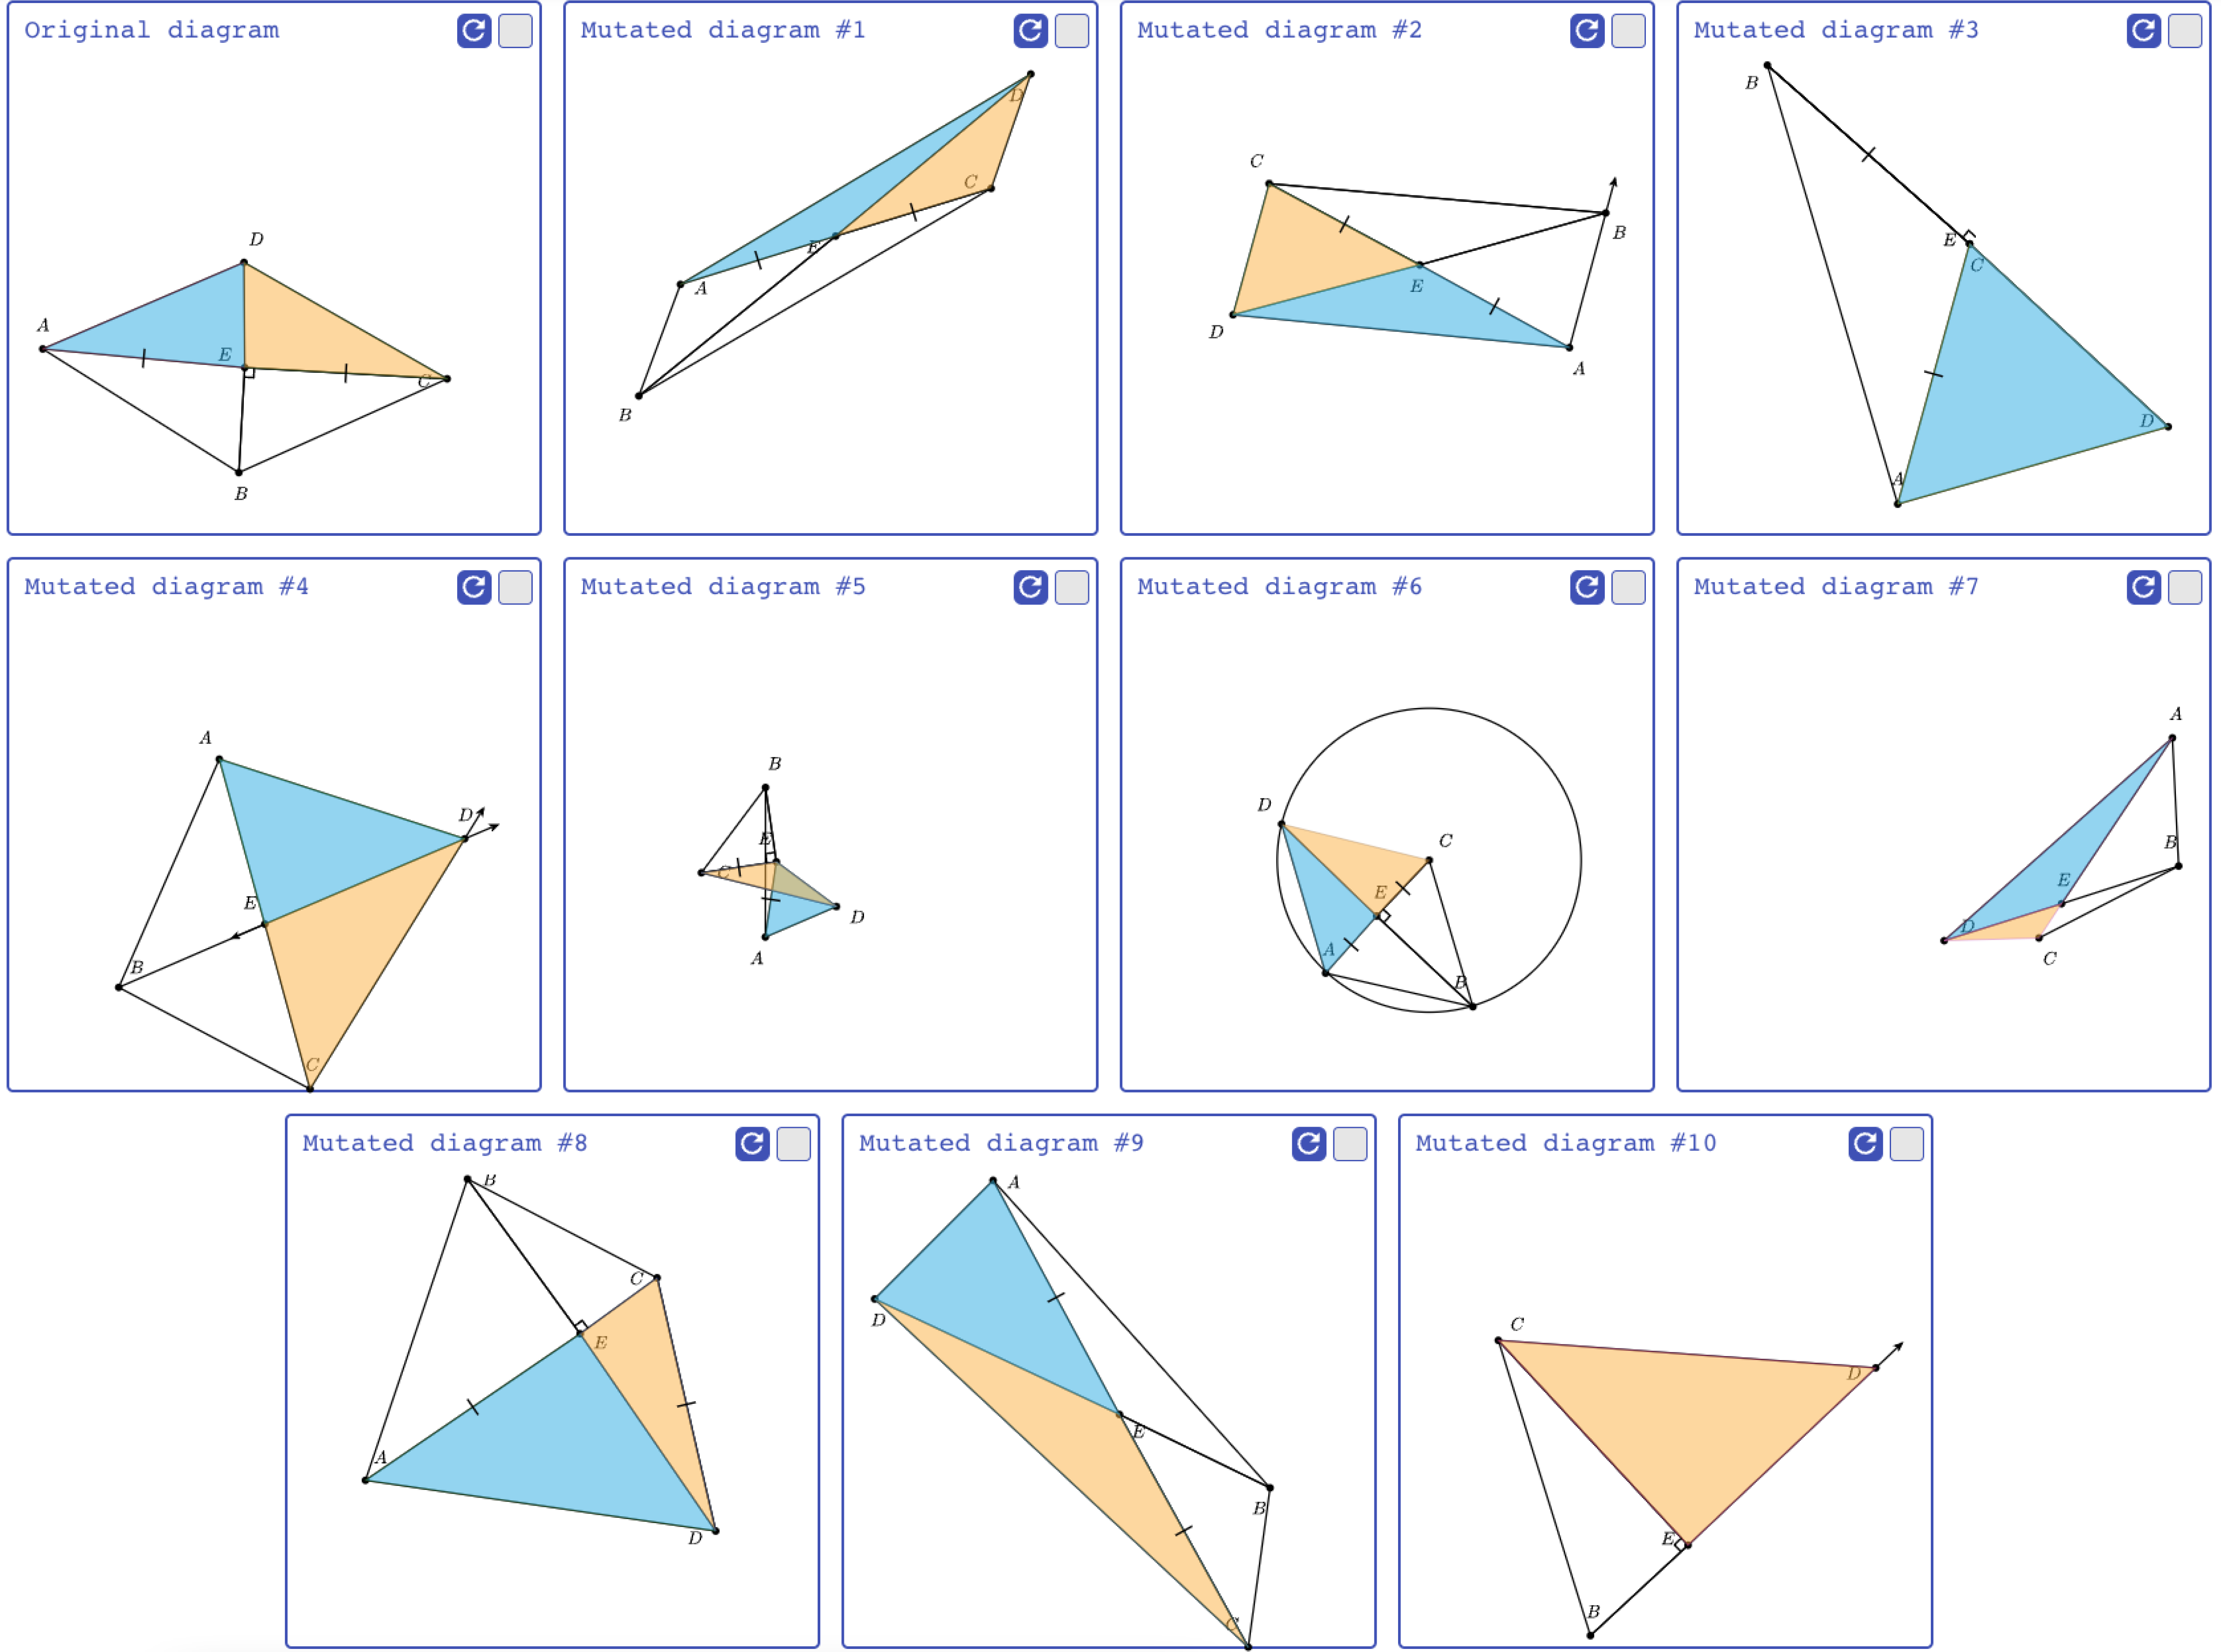
\includegraphics[width=\linewidth]{assets/chapter-3/geometry-grid.png}
    \caption{\textmd{The first ten diagram variations generated by \Edgeworth for the problem shown in \cref{fig:edgeworth-problems} (left).}}
    % \Description{This figure shows a grid of ten diagrams generated by Edgeworth given the example scenario in Figure 3 and 5. Some of the diagrams show congruent triangles DEA and DEC, while others show incongruent triangles.}
    \label{fig:geometry-grid}
\end{figure}

% \begin{figure}[h]
%     \centering
%     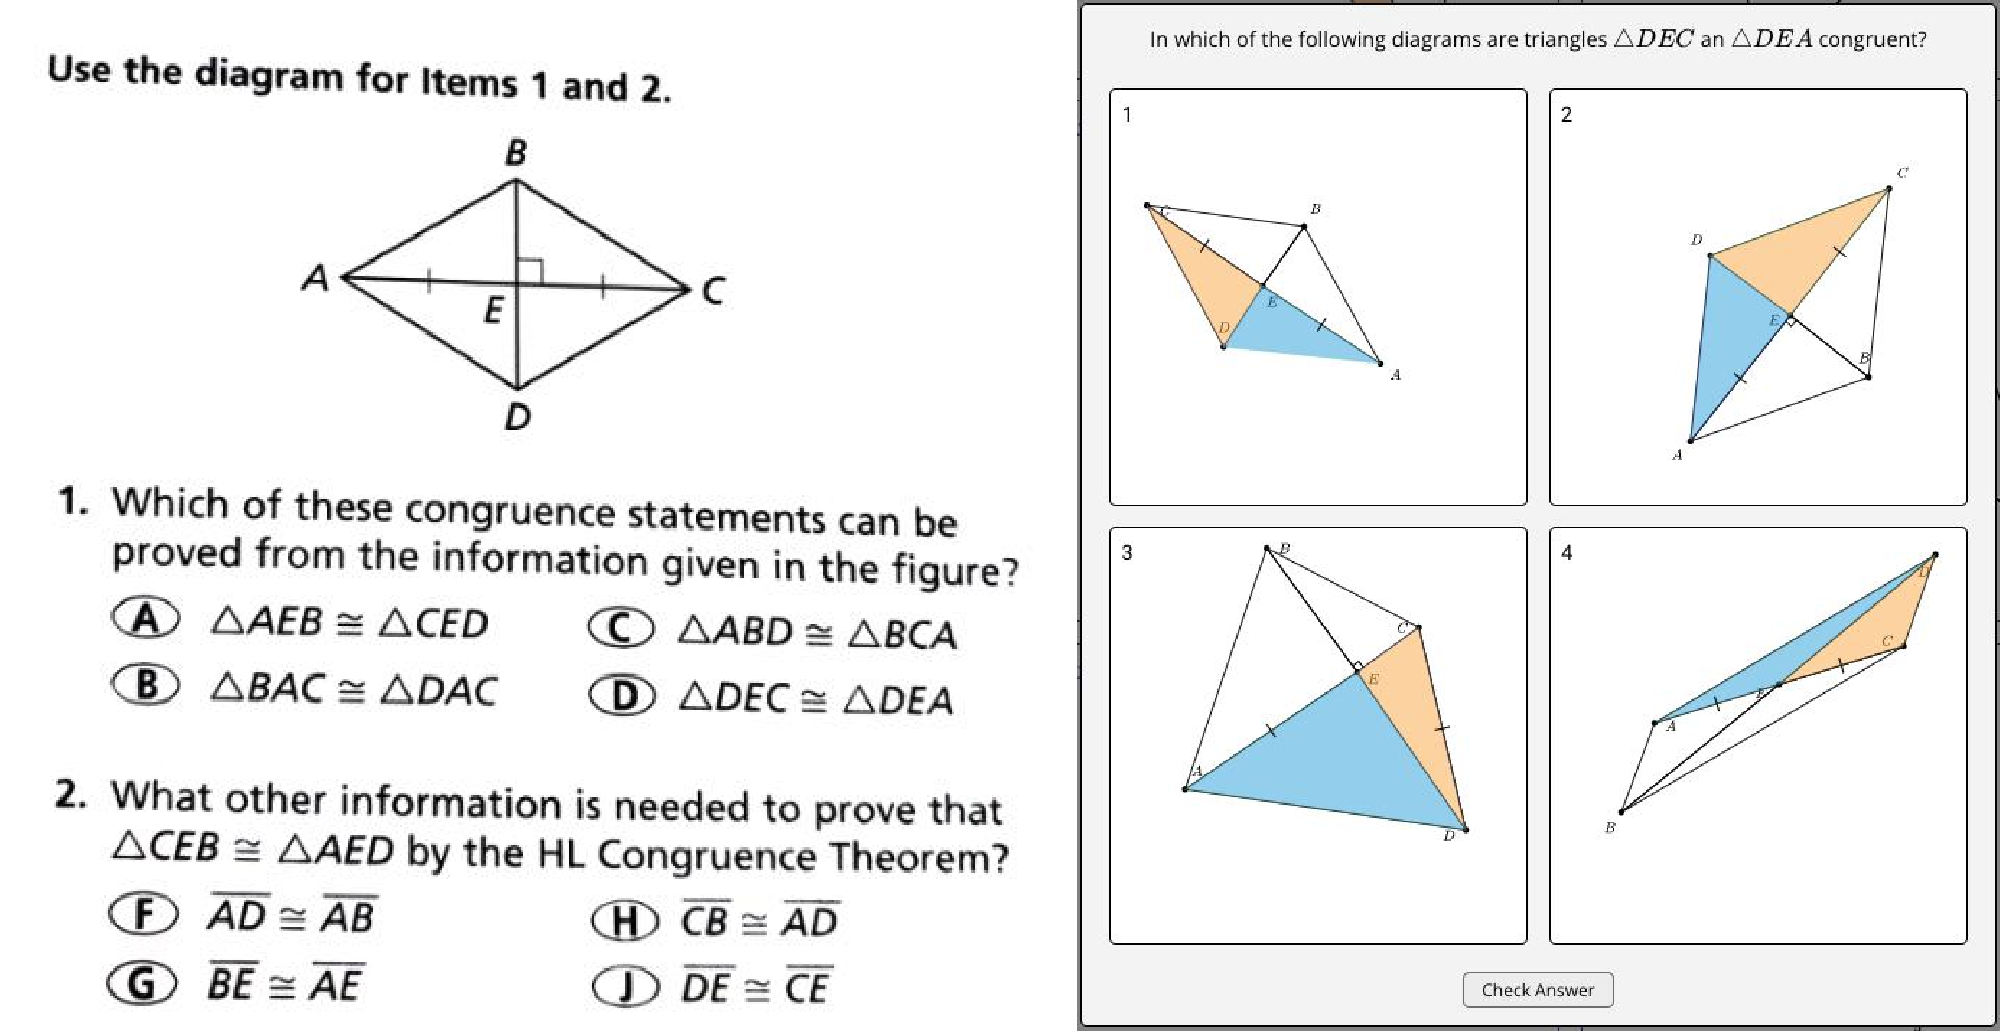
\includegraphics[width=\linewidth]{assets/geometry-problem.png}
%     \caption{An example problem in Holt \textit{Geometry}~\cite{burger2007holt} about triangle congruence (left) replicated in \Edgeworth (right). Colored shadings are added for clarity.}
%     \label{fig:geometry-problem}
% \end{figure}
We sample 17 Euclidean geometry problems from Holt \textit{Geometry} \cite{burger2007holt}, a high school geometry textbook. \cref{fig:edgeworth-problems} (left) shows an example problem. The textbook uses a consistent visual style of predominantly black line segments and dots with text labels. Most diagrammatic problems are presented as one diagram followed by one or more multiple-choice problems. We've recast the problems as diagrammatic translation problems.

For this domain, we build on the existing geometry stylesheet from \Penrose \cite[Section~5.3]{penrose} for diagram layout. In this domain, \Edgeworth weights deletions 20\% and edits 80\%. There are many different types of entities in geometry, so additions tend to introduce elements to the diagram that obviously do not pertain to the question prompt. Thus in this domain, the \Edgeworth mutator applies no additions. The reason we weight edits higher than deletions is that many of our geometry problems ask about specific named points, and deletions can make the diagram invalid by removing points that are mentioned in the prompt.

% \begin{wrapfigure}{r}{0.5\textwidth}
% \begin{figure}
%     \begin{center}
%         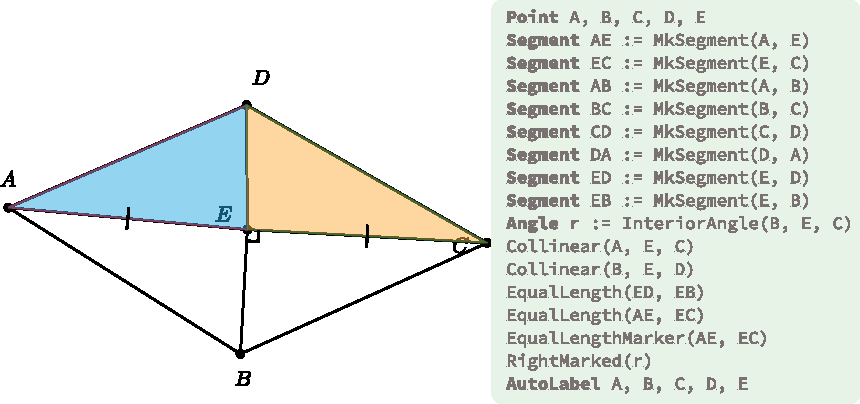
\includegraphics[width=\linewidth]{assets/congruence-example.pdf}
%     \end{center}
%     \caption{The example scenario of an Euclidean geometry problem.}
%     % \Description{This figure shows the diagram and Substance description of the example scenario in Figure 3. The diagram and Substance are identical to Figure 3.}
%     \label{fig:congruence-example}
% \end{figure}

% two-col
% \begin{figure}
%     \centering
%     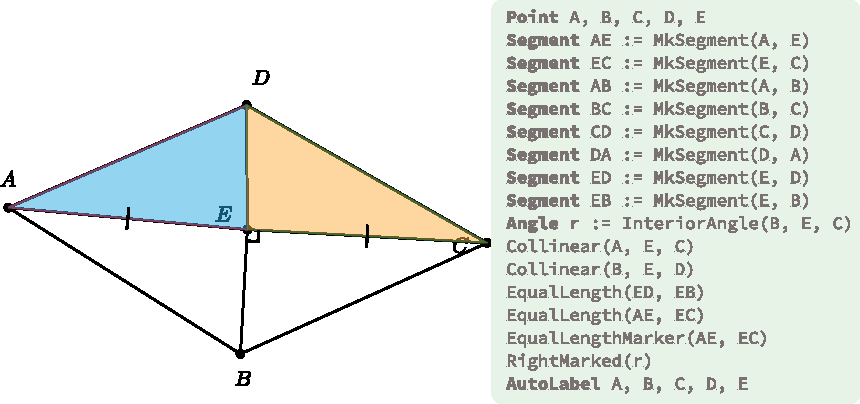
\includegraphics[width=\linewidth]{assets/congruence-example.pdf}
%     \caption{The example scenario of a Euclidean geometry problem.}
%     \Description{This figure shows the diagram and Substance description of the example scenario in Figure 3. The diagram and Substance are identical to Figure 3.}
%     \label{fig:congruence-example}
% \end{figure}

We use the problem in \cref{fig:edgeworth-problems} (left) to demonstrate how \Edgeworth generates variations that are meaningful as problem options. In the diagram shown, $\triangle DEC$ and $\triangle DEA$ are congruent by the Side-Angle-Side rule. In particular, they share a side ($DE$), the sides $AE$ and $EC$ appear to have equal length and are marked as such with a tick, and $\angle DEA$ and $\angle DEC$ are both right angles and therefore equal. 
% The diagram in \cref{fig:congruence-example} is replicated as Option 2 in \cref{fig:edgeworth-problems}. 
Option 4 in \cref{fig:edgeworth-problems} involves mutating the scenario by removing the right angle marker which makes it impossible to prove that $\angle DEA$ and $\angle DEC$ are equal. This is an example of the \textbf{Delete} mutation described in Section \ref{sec:edgeworth-mutation}. The angle appears to be a right angle in Option 3, so this option might serve as a good distractor for students still learning the distinction between the appearance of angles and their markings.

Option 3 involves mutating Option 2 by editing which sides have equal length. In Option 3, sides $CD$ and $AE$ are equal instead of $AE$ and $CE$. This is an example of the \textbf{Replace Arguments} mutation described in \cref{sec:edgeworth-mutation}. A student might incorrectly select Option 3 if they believed in a Side-Angle congruence rule, where a single angle and single side being equal could prove congruence. Finally, in Option 1 $\angle CEB$ neither is marked as a right angle nor appears as a right angle. A student might incorrectly select Option 1 if they believed in a Side-Side congruence rule, where two sides being equal could prove congruence.

\cref{fig:geometry-grid} shows the first 10 variations \Edgeworth generated from the example diagram. To create our problem, shown in \cref{fig:edgeworth-problems} (left), we selected the original diagram and two incorrect variations (numbers 1 and 8), plus another variation in an extended pool (number 16). As shown in \cref{fig:geometry-grid}, there are many other viable answer choices in the first 10 variations. Many of the diagrams involve extra details that are irrelevant to the problem, like the circle in number 6 or the vector above point B in number 2. These extra details can be pedagogically useful for teaching students to filter irrelevant information in the domain. Some of the other diagrams are very obviously incorrect, like number 10 which doesn't show a blue triangle, or number 7 where the blue triangle is much larger than the orange triangle; these can be useful for building confidence when students are first learning. 

% We assembled these problems from the diagrams alone. We did not look at the changes made to the textual scenario, and we do not expect our users to look at those textual changes. 

% \begin{figure}
%     \centering
%     \includegraphics[width=\linewidth]{assets/incorrect-mutants.pdf}
%     \caption{Three incorrect mutants (number 1, 8, and 16) selected for an Euclidean geometry problem (c04p01).}
%     \label{fig:incorrect-mutants}
% \end{figure}

% \cref{fig:incorrect-mutants} shows how \Edgeworth mutates the example scenario. For mutant 1, \Edgeworth changed \sub{RightMarked(r)} to make $\angle BEC$ an obtuse angle, thereby violating the SAS rule. The resulting diagram is visually obvious because the colored triangles clearly have different shapes. Mutant 8 violates another predicate \sub{EqualLength(AE, EC)} indirectly by changing the definition of $\overline{EC}$ to mean $\overline{CD}$. This is done by a combination of \textbf{Swap} and \textbf{Swap-In} mutations. The result is also a visually obvious incorrect diagram. Finally, mutant 18 changes \sub{RightMarked(r)} to \sub{RightUnmarked(r)} and also includes an irrelevant mutation that deletes $\overline{AD}$. Since the triangles are shaded, this extra mutation doesn't impact the readability of the resulting diagram. In fact, because $\angle BEC$ is still a right angle but not visually marked, it is a good distractor option for the problem. 




\subsection{General Chemistry: Lewis Structures}
\label{sec:chemistry}

% \begin{figure}[h]
%     \centering
%     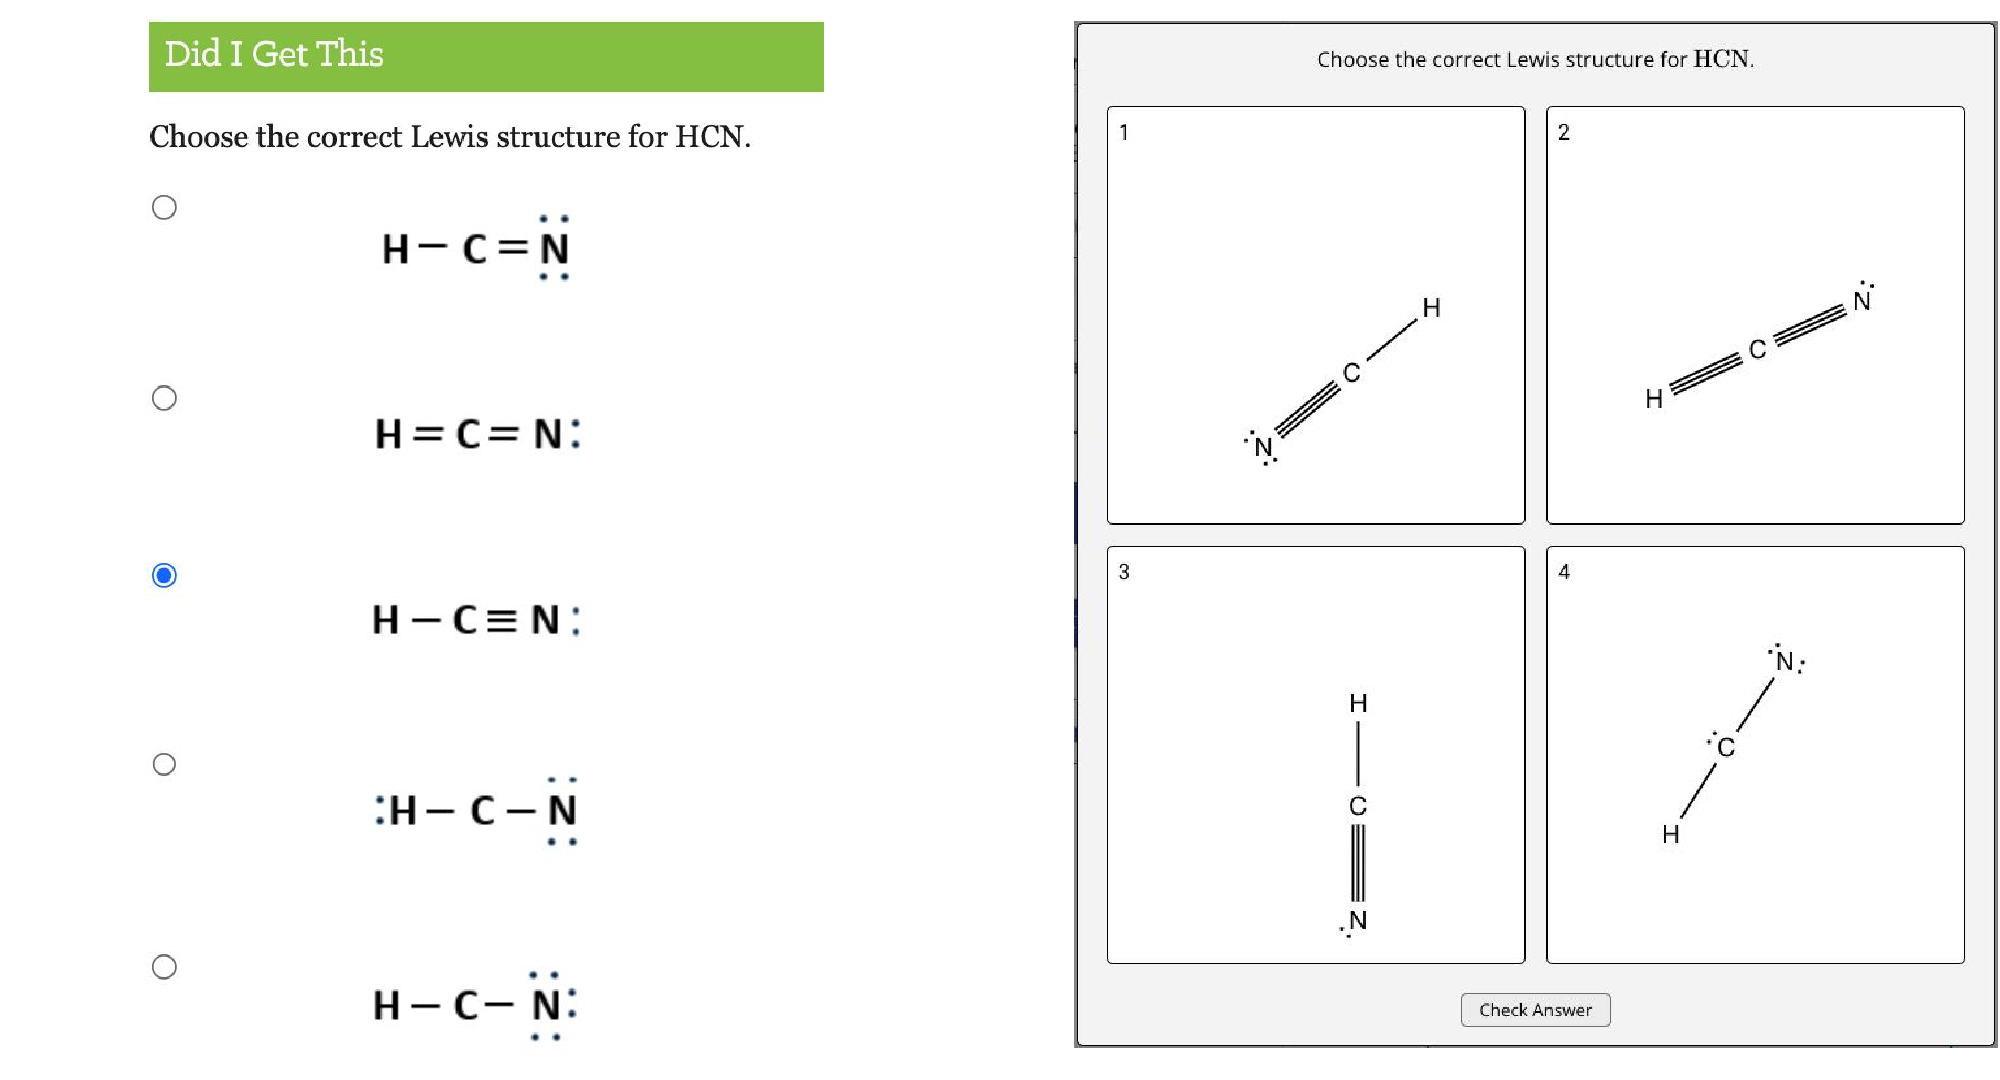
\includegraphics[width=\linewidth]{assets/chemistry-problem.png}
%     \caption{An example problem in general chemistry that asks the student to identify the correct Lewis structure for HCN.}
%     \label{fig:chem-problem}
% \end{figure}

We chose 7 chemistry problems on Lewis structure from an online General Chemistry 1 course \cite{oli}. These problems test students' understanding of how atoms bond together based on formal charges. The module introduces students to the \textit{octet rule}: the tendency of main group atoms to form enough bonds to obtain eight valence electrons. Lewis structure diagrams show bonds among atoms and valence electrons on atoms typically following the octet rule. 

% To accurately assess student understanding and give them appropriate varied practice, it is important that problems (and solution options) in this module differentiate student understanding of these more particular principles:

% \begin{itemize}
%     \item The number of valence electrons in the outer shell is determined by the atomic number.
%     \item The most common molecular configuration minimizes free electrons. 
% \end{itemize}

We extend the existing \Penrose chemistry stylesheet to include notation and layout rules for Lewis structures. To permit incorrect diagrams, the chemistry stylesheet must not enforce the octet rule. It does specify that an atom can have any number of bonds and that it can have 0, 2, 4, or 6 valence electrons. These specifications cover all problem scenarios in this Lewis structure module.\footnote{``Odd electron molecules are very rare and cannot achieve full octets of electrons around atoms because of the odd number of electrons.'' \cite{oli}} In accordance with stylistic conventions in the field, \Edgeworth automatically lays out atoms, bonds, and electrons to maximize bond angles and repel electrons from bonds 
% (\eg \cref{fig:cocl2-example} and \cref{fig:edgeworth-problems} bottom-middle)
. For molecules involved in all 7 problems, the layout algorithm produces high-quality diagrams without any manual manipulation needed from the author. 

To configure \Edgeworth for this domain, we weight edits 100\%. We exclusively weight on edits because we observed that variations of molecules never add or delete atoms and bonds. Although valence electrons may be added or deleted, they are modeled as predicates that can be edited to change the number of electrons for an atom (\eg \sub{ZeroDots(H)} $\rightarrow$ \sub{TwoDots(H)}) via a \textbf{Replace Function} mutation operation. 

Figure~\ref{fig:edgeworth-problems} (middle) shows an \Edgeworth Lewis structure problem for hydrogen cyanide, with the correct diagram in the top-left. Incorrect choices for this problem can be generated via mutation. For instance, if a student forgets that nitrogen must have eight surrounding electrons, they might choose the bottom-left option, which was generated by removing the valence electrons around nitrogen. Or, if a student does not know that hydrogen should only have two electrons instead of eight, they might select the top-right choice, which was generated by mutating the number of electrons around hydrogen from zero to six. Finally, if a student does not know that free electrons should be minimized, they might pick the bottom-right diagram, which was generated by mutating up the number of electrons around carbon and nitrogen and changing the triple bond to a double bond.

\subsection{Discrete Math: Graphs}
\label{sec:graphs}

% \begin{figure}[h]
%     \centering
%     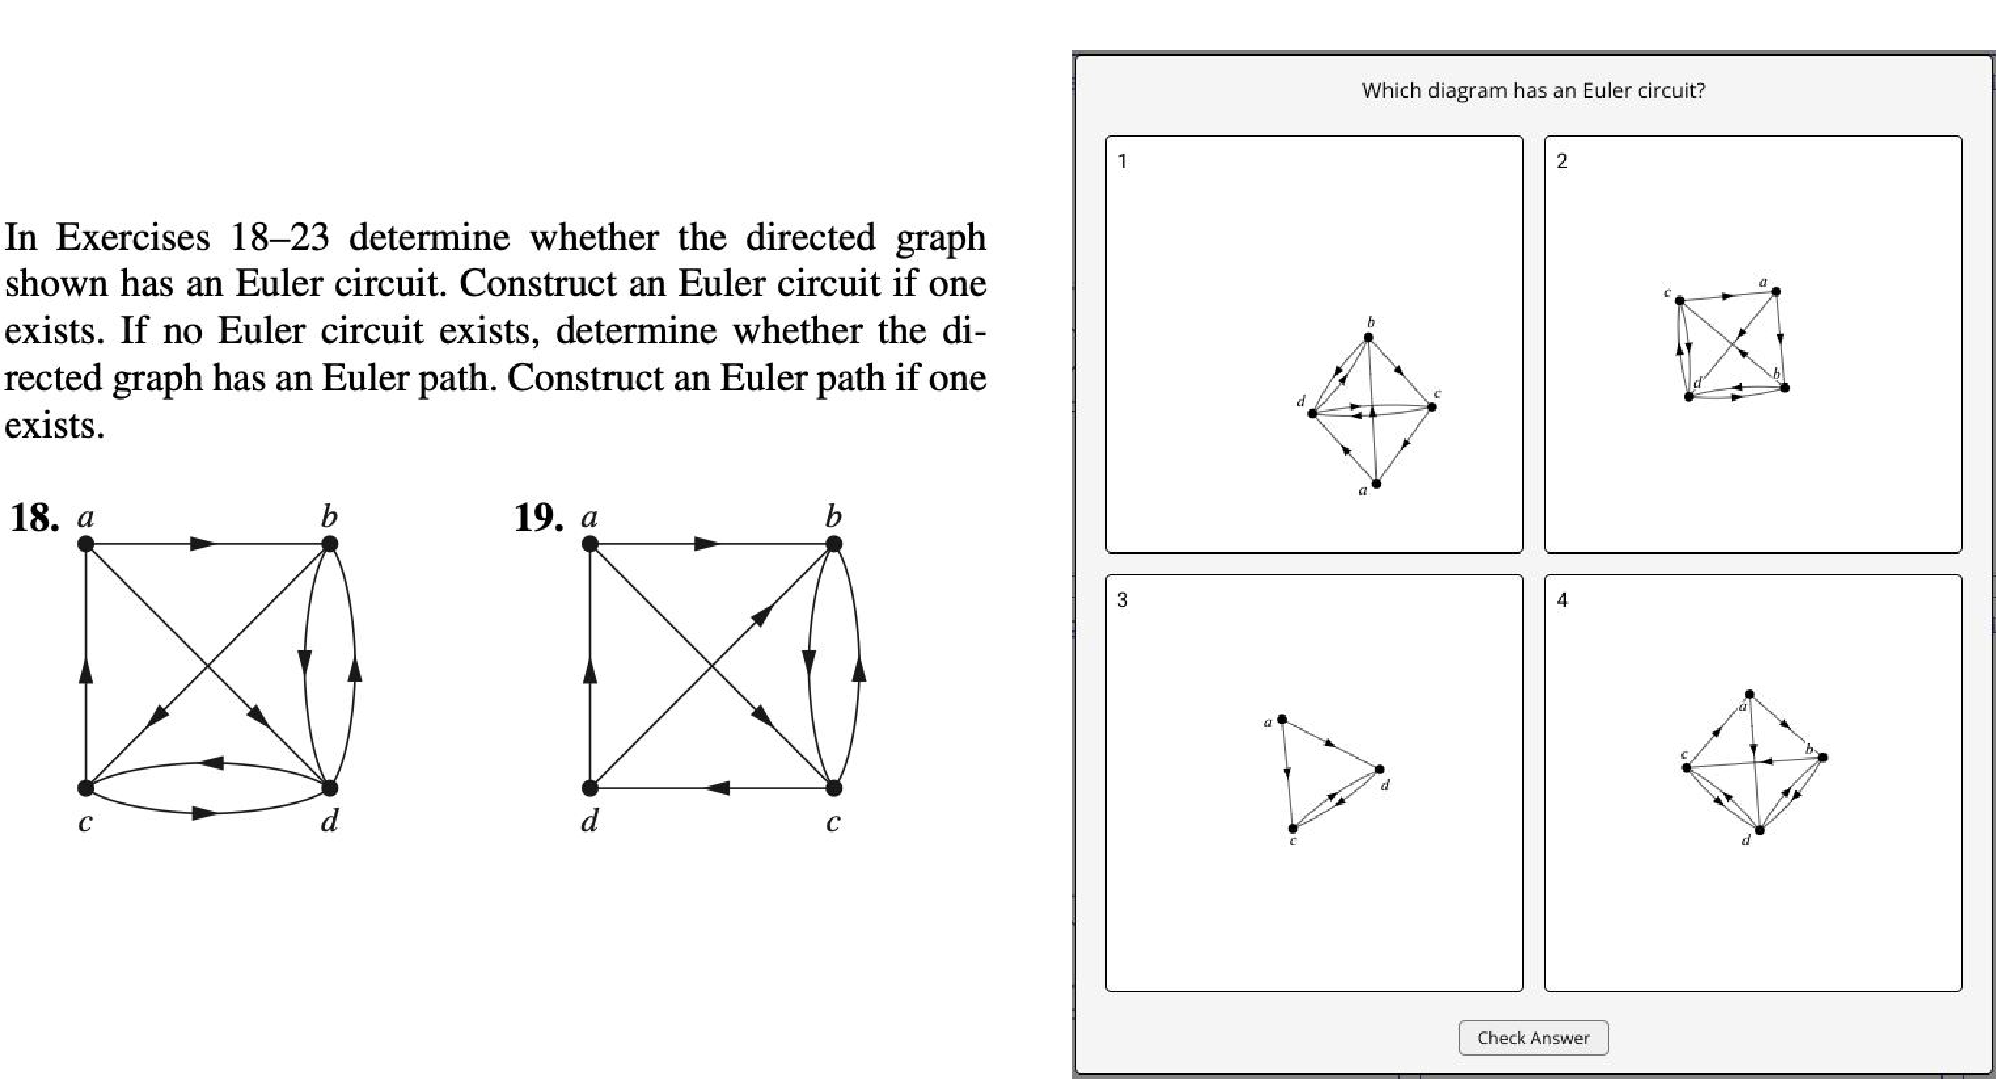
\includegraphics[width=\linewidth]{assets/graph-problem.png}
%     \caption{An example problem that asks the student to identify graphs with Euler circuits.}
%     \label{fig:chem-problem}
% \end{figure}

We draw 7 graph theory problems from the ``Graphs'' chapter of \textit{Discrete Mathematics and Its Applications} \cite[Chapter~10]{rosen1999discrete}.  We model our visual representation after the style used in the textbook, allowing students to recognize \Edgeworth-generated diagrams as they are already accustomed to recognizing graph diagrams. We created a new \Penrose stylesheet for four subdomains of graphs (directed vs not, and multigraph vs not). For each of these subdomains, \Edgeworth automatically lays out graph nodes, edges, loops, arrows, and labels in configurations that minimize confusing overlap of diagram elements. As with the other domains, no manual tweaking is necessary to obtain high-quality diagrams for problem variations. 
% The book defines six subdomains in Section 10.1, of which we use four:
% \begin{itemize}
%     \item \textit{Simple graph}---single undirected edges, no loops
%     \item \textit{Pseudograph}---multiple undirected edges, loops allowed
%     \item \textit{Simple directed graph}---single directed edges, no loops
%     \item \textit{Directed multigraph}---multiple directed edges, loops allowed
% \end{itemize}


To configure \Edgeworth for the graph domain, we weight additions 50\%, deletions 40\%, and edits 10\%. We disfavor edits in this domain because most of them are not useful: \textbf{Replace Function} is inapplicable for any of our graph subdomains, and \textbf{Swap Arguments} only applies to directed graphs. \textbf{Replace Arguments} is meaningful, but most desirable mutations for graphs are better represented by the addition or deletion of edges, or sometimes nodes. For instance, a bipartite graph can become not-so by adding edges, or a strongly-connected graph can become not-so by deleting edges. 

Figure~\ref{fig:edgeworth-problems} (right) shows an \Edgeworth problem asking which of four directed graphs have an Euler circuit. The bottom-right diagram does not have an Euler circuit, as can be seen by observing that the sum of $a$'s in-degree and out-degree is odd. In contrast, for the diagram in the bottom-left generated by deleting edge $(a, d)$, every node has an even sum of in-degree and out-degree, and indeed there does exist an Euler circuit. This condition on degree is only sufficient for undirected graphs, though; the diagram in the top-right is generated by flipping edge $(b, c)$ from the bottom-left diagram, but does not have an Euler circuit, thwarting the simple degree counting heuristic. Finally, the simple diagram in the top-left is generated by deleting $d$ and trivially has an Euler circuit. 

% \section{Summary}

% TODO

